\documentclass{article}
% TITLE PAGE CONTENT %%%%%%%%%%%%%%%%%%%%%%%%
% Remember to fill this section out for each
% lab write-up.
%%%%%%%%%%%%%%%%%%%%%%%%%%%%%%%%%%%%%%%%%%%%%
\usepackage{CJK}
\usepackage{float}
\usepackage{subfig}
\usepackage{graphicx}
\usepackage{listings} % For source cod
\usepackage{xcolor}
\usepackage{indentfirst}
\setlength{\parindent}{2em}
\usepackage{geometry}
\geometry{left=1.7cm,right=1.7cm,top=2.0cm,bottom=2.0cm}
\usepackage{float}
\usepackage{subfig}
% END TITLE PAGE CONTENT %%%%%%%%%%%%%%%%%%%%

\begin{document}  % START THE DOCUMENT!

\begin{CJK}{UTF8}{gkai}
\title{实验二 外腔半导体激光器特性测量}
\author{杨庆龙 \\1500012956}
\date{2018.9.26}
\maketitle

\section{实验目的}
\begin{enumerate}
  \item 熟悉认识半导体激光器电源的个模块及其功能;
  \item 理解外腔半导体激光器输出频率的连续调谐与跳模;
  \item 理解外腔半导体激光器输出功率的电调特性与温调特性;
  \item 通过示波器观察激光的纵模,并感受半导体激光器模式竞争过程;
  \item 学习使用波长计,并测量激光器输出激光的波长。
\end{enumerate}

\section{实验内容}
\subsection{测量阈值电流}
按照激光器操作流程,打开激光器,并将激光器温度设置到20摄氏度。待激光器正常工作并温度稳定后,从20mA开始,逐步增大激光器电流,并待激光器纵模稳定后,记录下软件上的功率读数,可得表格\ref{t1.0}并绘制电流功率图\ref{f1.0}。\\
\begin{table}[H]
  \centering
  \caption{阈值电流测量数据记录表}
  \label{t1.0}
\begin{tabular}{|c|c|c|c|c|c|c|c|c|c|}
  \hline
  电流/mA&20&24&27&28&29&30&31&32&34\\
  \hline
  功率/mW&0.00101&0.00101&0.00101&0.00222&0.00915&0.0144&0.0181&0.0238&0.0274\\
  \hline
  电流/mA&38&42&44&46&50&54&57&61&\\
  \hline
  功率/mW&0.0483&0.0626&0.0658&0.0988&0.114&0.118&0.132&0.137&\\
  \hline
\end{tabular}
\end{table}
\indent 绘制出激光器的电流功率曲线并进行线性拟合后,可以计算得出该激光器的阈值电流约为25.31mA。观察电流功率图,可以发现在输入45mA电流时,曲线发生了较大波动。经过讨论与测试之后得出结论,这是由于同学在操作激光器时对桌子施加了较大的力量,导致桌面发生严重形变,引起光路发生变化,使得射入波长计的光强发生变化,最终导致功率示数发生突变。

\begin{figure}[H]
  \centering
  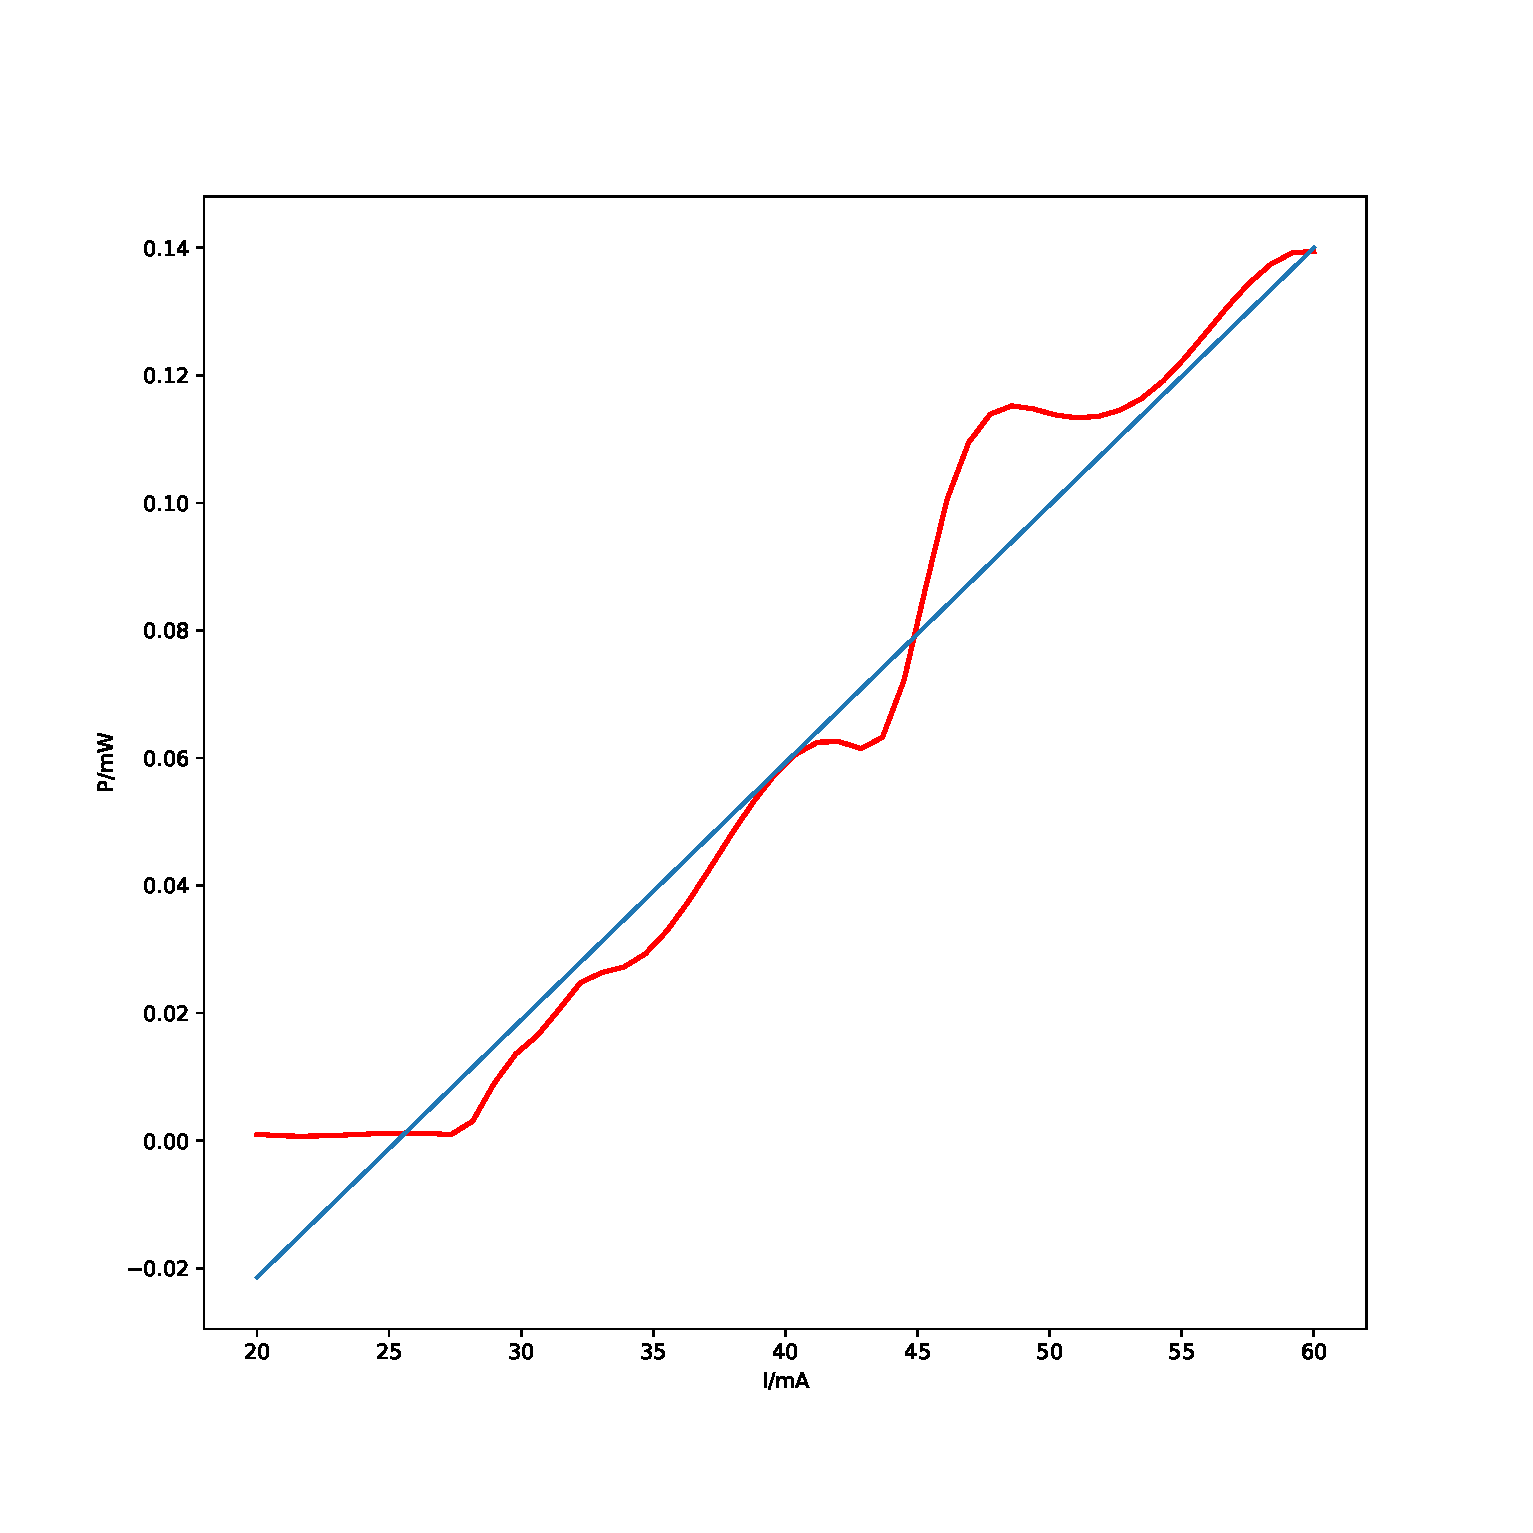
\includegraphics[width=0.4\textwidth]{exm1_1.eps}
  \caption{电流-功率曲线图}
  \label{f1.0}
\end{figure}

\subsection{测量外腔半导体激光器频率的温调特性}
将激光器电流设置为40mA,再将半导体的温度从20.0摄氏度开始,以0.3摄氏度的步长增加到23.0摄氏度。并在每次改变温度后等待激光器稳定,并记录波长数据,得到表格\ref{t2.1},绘制得到该激光器的温调特性曲线\ref{f2.1}。
\begin{table}[H]
\centering
  \caption{激光器频率温调实验数据记录表}
  \label{t2.1}
  \begin{tabular}{|c|c|c|c|c|c|c|c|c|c|c|c|c|c|}
    \hline
    温度/摄氏度&20&20.3&20.6&20.9&21.2&21.5\\
    \hline
    波长/纳米&780.431&780.448&780.371&780.386&780.404&780.421\\
    \hline
    温度/摄氏度&21.8&22.1&22.4&22.7&23.0&\\
    \hline
    波长/纳米&780.436&780.452&780.378&780.392&780.411&\\
    \hline
  \end{tabular}
\end{table}
\begin{figure}[H]
  \centering
  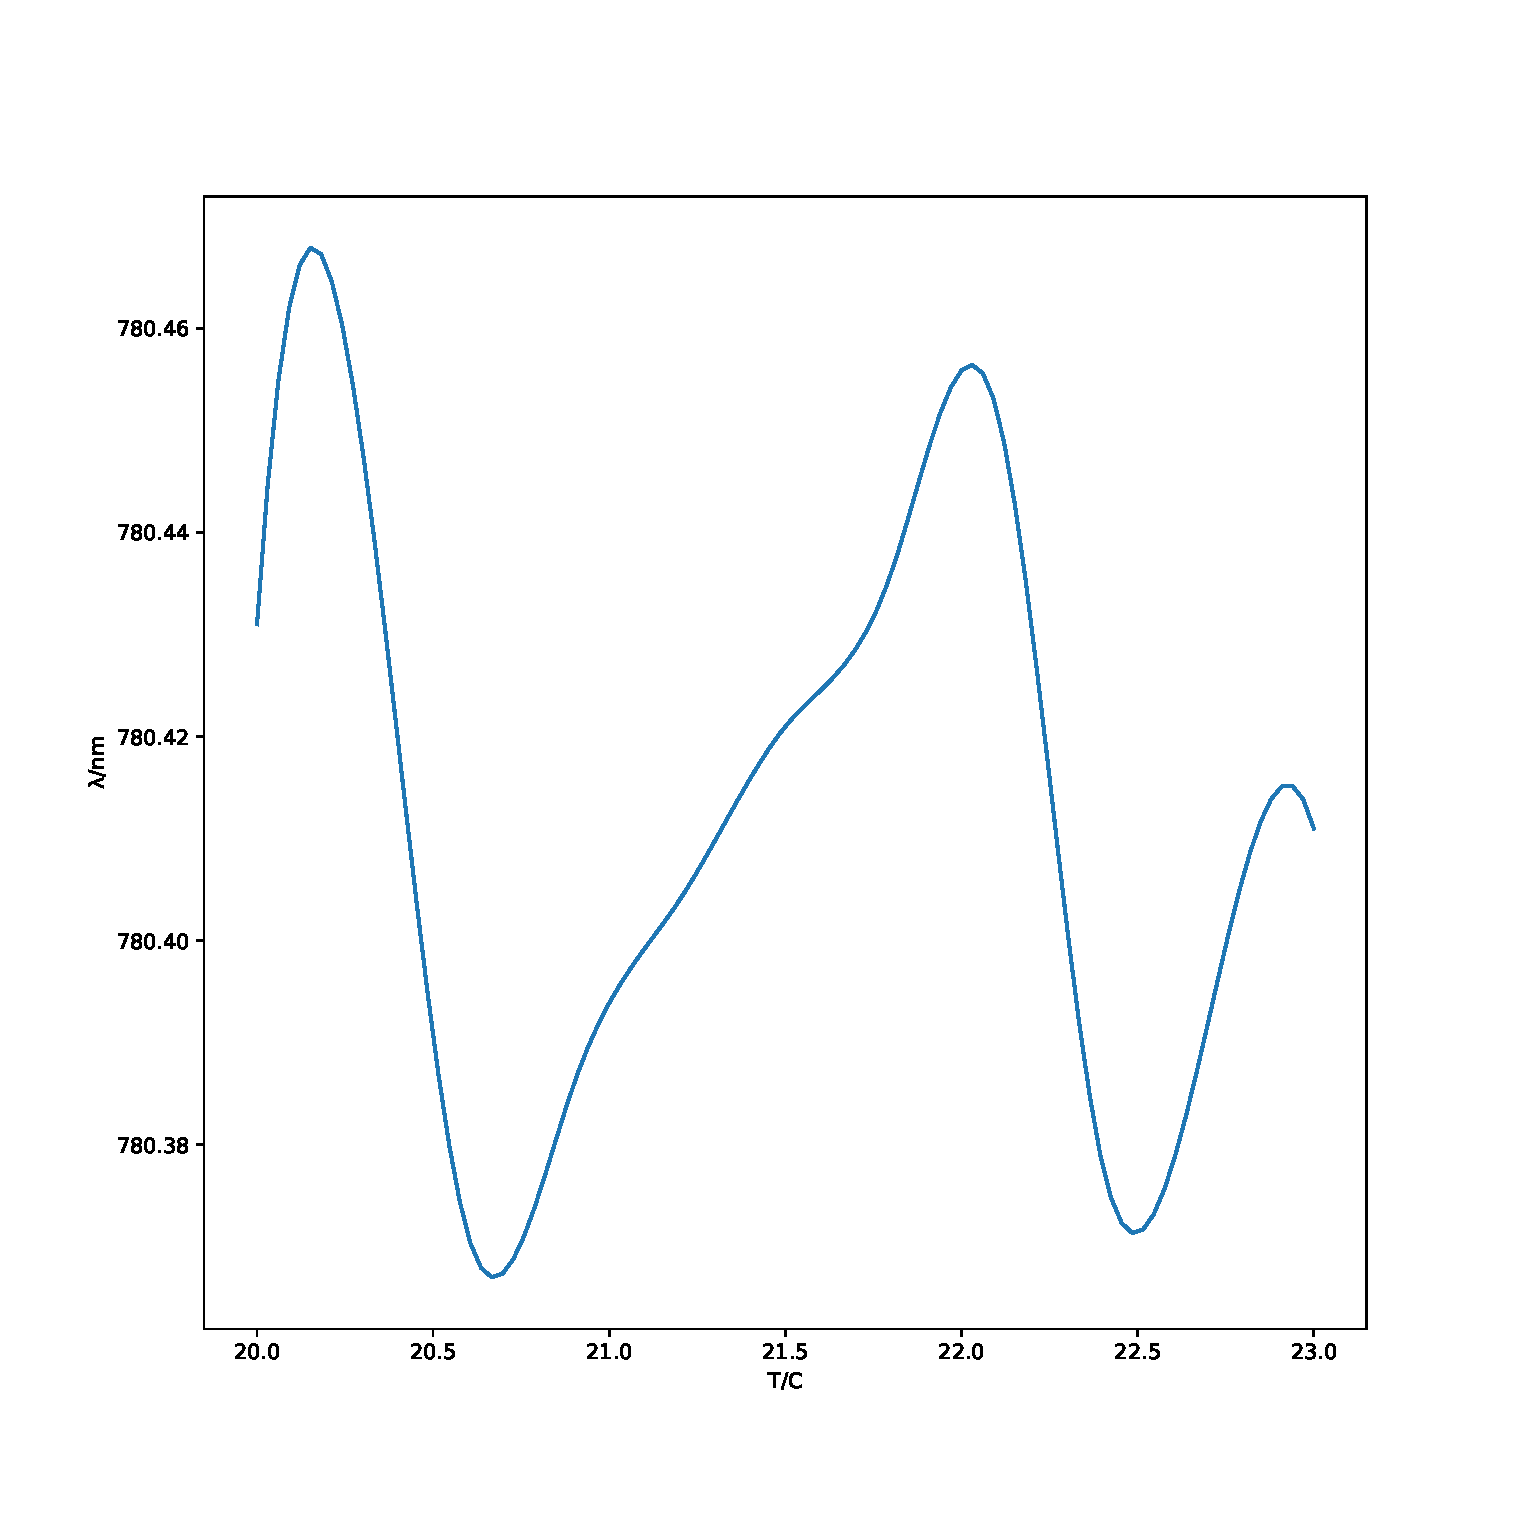
\includegraphics[width=0.4\textwidth]{exm1_3.eps}
  \caption{温度-频率曲线图}
  \label{f2.1}
\end{figure}
\indent 从温调曲线图中可以看到,该激光器的输出波长随着温度的上升也会发生跳模现象,在20.0摄氏度到23.0摄氏度的范围内,跳模现象之间约间隔2.0摄氏度。但是,该曲线同时表明,激光器的波长一直维持在780.37纳米到780.45纳米之间,并未表现出理论上的每次跳模都会带来波长阶跃的现象。要解释该现象需要先了解有哪些参数影响着激光器的发射频率.\\
\indent 首先,半导体激光器内部的PN结会同时产生不同频率的激光,这些激光线宽很宽,且互相之间有着一定间隔;其次,对于Littrow型激光器,闪耀光栅会将不同频率的光反射到不同的角度上,只有一定范围内的光可以射回到激光器进行放大,而放大过的光线强度远大于其他频段的光,这就对发射频率进行了一次筛选;最后,再由激光器外腔对闪耀光栅反射出的光线进行筛选,而外腔对光线频率的限制很明显,只有满足一定波长条件的光线能够射出外腔,否则就会被外腔消耗掉,这就完成了最后一次频率限制。\\
\indent 在我们的实验过程中,闪耀光栅的角度和外腔长度自始至终都没有发生过变化,这也就导致射出光线的频率只会是闪耀光栅反射回激光器的频段与能通过外腔的频率的交集,进而导致激光器的射出光线频率总是维持在一定的范围内。又因为PN结发射出的激光频率会发生跳变,每次跳变都会使得新的模式进入到放大频段里,进而导致实验中每次跳模都使得射出激光器的光线频率从一个较长的波长改变至一个较短的波长。


\subsection{激光器频率电调实验}
调节半导体激光器的温度模块,将温度设定在20.0摄氏度,待温度稳定后,从阈值电流开始,逐步增大电流,直到阈值电流的三倍。记录实验数据可得表\ref{t3.1},并作出电流频率曲线\ref{f2.1}。\\
\begin{table}[H]
\centering
  \caption{激光器频率电调实验数据记录表}
  \label{t3.1}
  \begin{tabular}{|c|c|c|c|c|c|c|c|c|c|c|}
    \hline
    电流/毫安&28&29&30&31&32&34&38&42&44&46\\
    \hline
    波长/纳米&780.374&780.375&780.386&780.386&780.397&780.398&780.421&780.432&780.444&780.360\\
    \hline
    电流/毫安&50&54&57&61&65&69&73&76&81&\\
    \hline
    波长/纳米&780.384&780.407&780.419&780.443&780.372&780.395&780.419&780.430&780.371&\\
    \hline
  \end{tabular}
\end{table}
\begin{figure}[H]
  \centering
  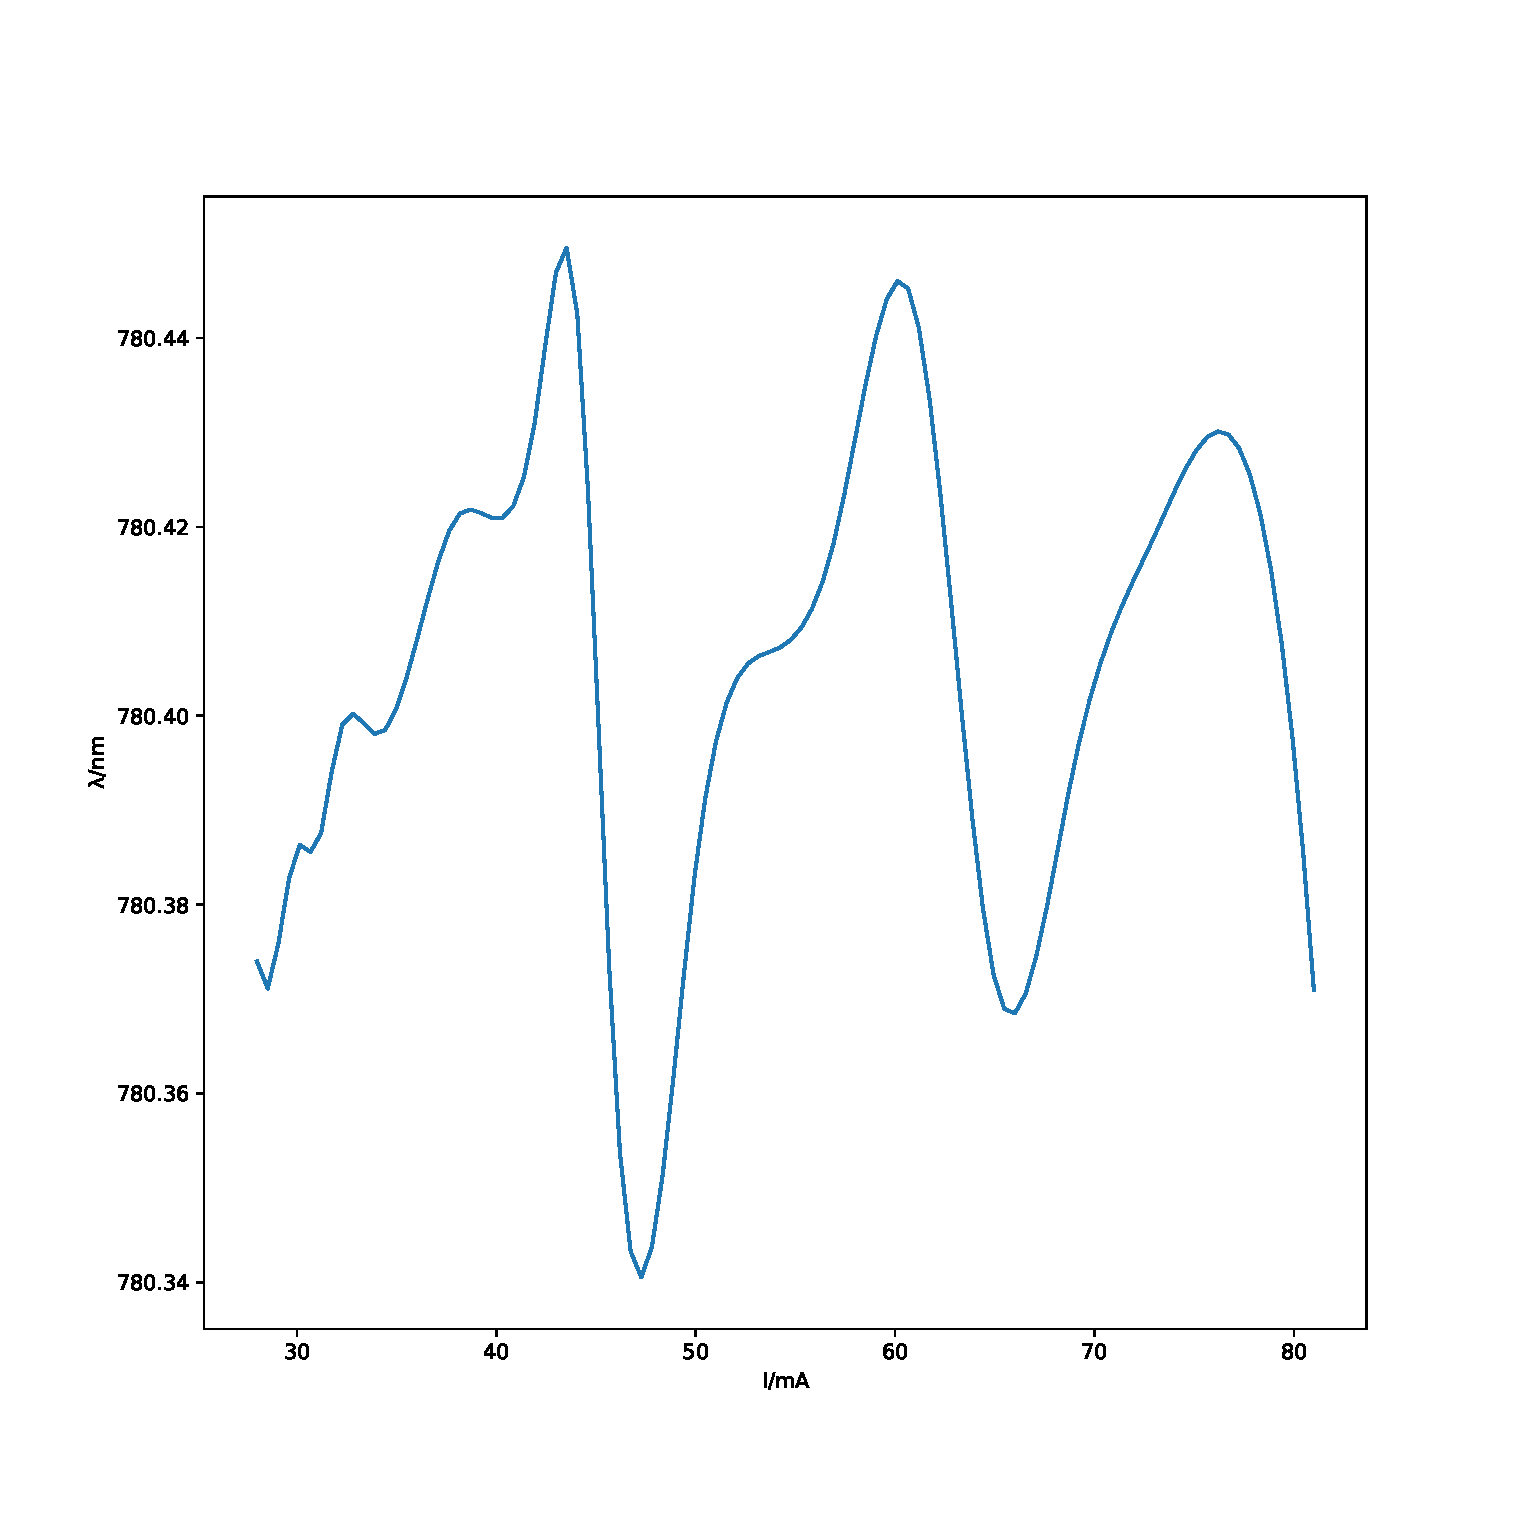
\includegraphics[width=0.4\textwidth]{exm1_2.eps}
  \caption{电流-频率曲线图}
  \label{f2.1}
\end{figure}
\indent 从电流频率曲线可以看到,在约37mA电流之前,激光器表现出期望的跳模现象,及在一定电流范围内波长稳定,但增大到一定程度就会导致波长突然变长。但到了37mA之后,由于闪耀光栅和外腔对波长的控制,导致输出波长变短,之后由于波长还未超出限制范围,所以依然能看到正常的跳模现象,直到波长超过限制范围。
\section{思考题}
\subsection{对外腔半导体激光器来说,有哪些频率调谐的方式?}
对于实验所用的外腔半导体激光器来说,频率调谐方式有
\begin{enumerate}
  \item 改变激光器的输入电路
  \item 改变激光器的工作温度
  \item 改变闪耀光栅的角度
  \item 改变外腔长度
\end{enumerate}
\subsection{计算电调率和温调率,并与第一章数据进行比较?}
通过实验数据计算得出该激光器的温调率约为21GHz/K,而电调率为800MHz/mA,和第一章给的数据略有偏差。


\end{CJK}

\end{document} % DONE WITH DOCUMENT!
